\documentclass{report}

\usepackage{amsmath}
\usepackage{amssymb}
\usepackage{amsthm}


\newtheorem{theorem}{Theorem}[chapter]
\newtheoremstyle{exampstyle}
  {\topsep} % Space above
  {\topsep} % Space below
  {} % Body font
  {} % Indent amount
  {\bfseries} % Theorem head font
  {.} % Punctuation after theorem head
  {.5em} % Space after theorem head
  {} % Theorem head spec (can be left empty, meaning `normal')
\theoremstyle{exampstyle} \newtheorem{example}[theorem]{Example}
\theoremstyle{exampstyle} \newtheorem{remark}[theorem]{Remark}
\theoremstyle{exampstyle} \newtheorem{definition}[theorem]{Definition}
\theoremstyle{exampstyle} \newtheorem{lemma}[theorem]{Lemma}

\usepackage[english]{babel}
\usepackage{csquotes}
\usepackage{graphicx}
\usepackage{verbatim}
\usepackage{listings}
\usepackage{float}
\usepackage{dsfont}
\usepackage[width=6in, height=8in]{geometry}
\usepackage{xcolor}

\usepackage[
backend=biber,
natbib=true,
url=false, 
doi=true,
eprint=false
]{biblatex}
\addbibresource{sources.bib}

\definecolor{codegreen}{rgb}{0,0.6,0}
\definecolor{codegray}{rgb}{0.5,0.5,0.5}
\definecolor{codepurple}{rgb}{0.58,0,0.82}
\definecolor{backcolour}{rgb}{0.95,0.95,0.92}

\lstdefinestyle{mystyle}{
	backgroundcolor=\color{backcolour},   
	commentstyle=\color{codegreen},
	keywordstyle=\color{magenta},
	numberstyle=\tiny\color{codegray},
	stringstyle=\color{codepurple},
	basicstyle=\ttfamily\footnotesize,
	breakatwhitespace=false,         
	breaklines=true,                 
	captionpos=b,                    
	keepspaces=true,                 
	numbers=left,                    
	numbersep=5pt,                  
	showspaces=false,                
	showstringspaces=false,
	showtabs=false,                  
	tabsize=2
}

\lstset{style=mystyle}

\begin{document}



\chapter{Positivity Preservation}

\section{Positive Solutions to ODEs}

\subsection{Motivation}

There are many problems which motivate the need for numerical methods which preserve positivity of the solution.
For example, consider the problem of simulating a chemical reaction.
We start with a finite amout of positive-valued species at the initial stage, and apply some numerical method to produce a result.
Despite being able to apply methods which have high orders of accuracy, traditional methods will not preserve positivity unconditionally.
If our numerical solution indicates that the concentrations of any number of species become negative, then our solution is not qualitatively accurate to a ``true'' solution.

Consider a problem given by $\dot{x} = f(x)$, with the initial condition $x(0) = x_0$.
For a one-dimensional problem, the true solution is positive if, given $x_0 \ge 0$, we have that $x(t) \ge 0$ for $t>0$.
Positivity of the numerical solution can be expressed as the condition that if $x_i \ge 0$ then $x_{i+1} \ge 0$ for all $i = 1, \mathellipsis, N$ timesteps in the computation.
Like always, $x$ may be vector-valued. If $x \in \mathds{R}^d$,
then the condition for positivity of the numerical solution applies element-wise to each component $x_i^{(k)}$ for $k = 1, \mathellipsis, d$.
Importantly, entries \textit{can} be zero. 

Methods which preserve positivity are a current area of research. It is difficult to produce numerical methods which both preserve positivity and maintain high order accuracy.
Moreover, it is very difficult to formulate positivity preserving methods for general problems.
Our approach will be to consider particular cases, where we can reduce the problem $\dot{x} = f(x)$ to a particular form,
and formulate positivity-preserving methods which are effective for these problems.

\subsection{The Graph-Laplacian Matrix}

Before looking at positivity-preserving methods, we will consider problems which themselves must admit positivity-preserving solutions.
The notion of the graph-Laplacian matrix and the methods centered around it are taken from \cite{blanes_pos_2022}.

Our main focus will be on problems that we can write in the form 
\begin{equation*}
    \dot{x} = A(x)x
\end{equation*}
where $A$ is a graph-Laplacian matrix.

\begin{definition}
    A graph-Laplacian matrix $A \in \mathds{R}^{d \times d}$ is a square matrix that satisfies
    \begin{itemize}
        \item $\mathbf{1}^\intercal A = \mathbf{0}^\intercal ~~ \text{(its column sums are zero)}.$
        \item For all $i, j = 1, \mathellipsis, d$ where $i \ne j$ we have $A_{ij} \ge 0$.
        \item For all $i = 1, \mathellipsis, d$ we have $A_{ii} \le 0$
    \end{itemize}
\end{definition}

Note that here, $A$ can depend on $x$. The entries in $A(x)$ can contain entries of $x$ in any fashion, as long as the definition is satisfied.

\begin{example}
    The Robertson reaction, taken from \cite{blanes_pos_2022}, is given by the matrix equation
    \begin{equation*}
        \frac{\mathrm{d}}{\mathrm{d}t}\begin{pmatrix}
            x_1 \\
            x_2 \\
            x_3
        \end{pmatrix} = \begin{bmatrix}
            -0.04 & 10^4 x_3 & 0 \\
            0.04 & -3\times 10^7 x_2 - 10^4 x_3 & 0 \\
            0 & 3 \times 10^7 x_2 & 0
        \end{bmatrix} \begin{pmatrix}
            x_1 \\
            x_2 \\
            x_3
        \end{pmatrix}.
    \end{equation*}
    This is a matrix equation of the form $\dot{x} = A(x)x$, where $A$ is a graph-Laplacian matrix.
    This problem describes a chemical reaction of three species.
\end{example}

The name ``graph-Laplacian'' comes from graph theory, and the definition is not universally agreed upon.
For our needs, we consider a graph-Laplacian matrix for a directional graph to be the in-degree matrix (diagonal) minus the in-degree adjacency matrix (empty diagonal) of the graph.
If a problem admits the reduction to graph-Laplacian form like the above,
we can show that the solution retains positivity.

\begin{theorem}
    Solutions of $\dot{x} = A(x)x$ retain positivity if $A$ is graph-Laplacian.
\end{theorem}
\begin{proof}
    Consider the solution $x(t^*)$ at time $t^*$. Assume that there are indices $k \in \{1,\mathellipsis, d\}$ where all entries $x_k(t^*)$ are zero and the rest are strictly positive.
    Then the $k$-th equation in the matrix system is
    \begin{equation*}
        \dot{x}_k(t^*) = \sum_{l = 1}^{d} A_{kl}(x(t^*))x_l(t^*).
    \end{equation*}
    Entry $A_{kk}$ is negative, but we assumed $x_k(t^*)=0$ so the only contributions to the sum are the $A_{kl}$ and $x_l$ for $l \ne k$.
    Some of the $x_l$ may be zero but all the rest are positive, so we have $\dot{x}_k \ge 0$.
    Note that equality is attained if all the $x_k$ are zero which is the trivial solution. 
    Assume instead that every entry $x_k(t^*)$ is non-zero and hence positive.
    In this case there are no restrictions on the derivative of the $k$-th entry - the $A_{kk}$ term means this derivative can be negative.
    The $x_k$ term can go to zero, but since the derivative is strictly non-negative at zero, we will retain positivity.
\end{proof}

We have shown that the graph-Laplacian form is a suitable structure for problems where we are concerned about positivity preservation.
From now on, for a vector solution $x \in \mathds{R}^d$ we will write $x \ge 0$ to mean that each element $x_k \ge 0$ for $k = 1, \mathellipsis, d$.
Before moving on to numerical methods that preserve positivity of these problems, we will consider a few points of note.

\subsection{Non-autonomous Systems}

Our analysis so far has focused on problems $\dot{x} = A(x)x$, which are autonomous.
Examples in positivity preservation can often be non-autonomous, which we would write as $\dot{x} = A(x,t)x$.
The particular details of problems involving the graph-Laplacian matrix can be easily analogised to the non-autonomous case.
As such, we will usually only consider problems in the autonomous form, unless it is necessary to the analysis.

Some problems can involve several different timescales,
in which case time-dependence is very important to account for.

\subsection{Conservation of Mass}

%% how graph laplacians also maintain conservation of mass and why this is nice.

When problems describe an exchange of matter, it is useful for this matter to be conserved in our solution.
Conservation of mass is the condition that $x$ satisfies $\mathbf{1}^\top x = C$ for some constant $C$.
Mass is conserved for graph-Laplacian problems because
\begin{equation*}
    \frac{\mathrm{d}}{\mathrm{d}t}\mathbf{1}^\top x = \mathbf{1}^\top \dot{x} = \mathbf{1}^\top A(x)x = \mathbf{0}^\top x = 0
\end{equation*}
hence clearly $\mathbf{1}^\top x$ is constant.
In the literature we often have $C=1$ for simplicity,
there is no loss of generality because this can be applied to some scaling of the initial condition such that $\mathbf{1}^\top x_0 = 1$.

Mass preservation can be generalised to higher order problems involving inner products with the variable of interest.
These problems concern conservation of other properties, which we will not explore in depth.

\section{Positivity Preserving Methods}

% maybe leave this bit for later
\subsection{Brute force approach}

Before considering the problem of positivity preserving methods in depth, we will first consider the method which we will refer to as ``fixing''.
We use the forward Euler method $x_{i+1} = x_i + hf(x_i)$, except at every step we perform a fix by considering every entry in $x_i$ and if it is negative, we just set it to zero.
We can write this formally as the method
\begin{align*}
    x_{i+1} &= x_i + h f(x_i) \\
    x_{i+1} &= \mathcal{H}_+(x_{i+1}) 
\end{align*}
where $\mathcal{H}_+$ is the thresholder that sets all negative entries to zero.
This is equivalent to a projection of $x$ to a vector subspace of lower dimension, determined by in which dimensions $x$ is positive.

This method is very cheap, and it preserves positivity, so it seems like an easy choice.
The fixing step to eliminate negative entries can be applied in general to any numerical method.
%discuss a result

Euler's method serves as a useful baseline to demonstrate experimental ideas.
Being a first-order accurate method, it does not serve as an effective choice for general applications.
We will instead look at different approaches to preserving positivity of the numerical solution,
using the graph-Laplacian structure explored earlier.

\subsection{General Solutions}

Consider the problem $\dot{x} = Ax$, with initial condition $x(t=0) = x_0$, with a constant square matrix $A$.
The general solution to this problem is
\begin{equation*}
    x(t) = \mathrm{e}^{tA} x_0
\end{equation*}
where the matrix exponential is analogised from the scalar case
\begin{equation*}
    \mathrm{e}^A = I + A + \frac{1}{2}A^2 + \frac{1}{6}A^3 + \mathellipsis = \sum_{j=0}^{\infty} \frac{A^j}{j!}.
\end{equation*}
We have shown that in the case where $A$ is graph-Laplacian, solutions preserve positivity.

We can't immediately apply this exponential solution to the problem $\dot{x} = A(x)x$ because of the non-linear right hand side, which will lead to a different expansion via. product rule.
To see why, we will demonstrate the expansion. Assume that the solution for the graph-Laplacian problem is $x(t) = \exp(tA(x))x_0$.
Then
\begin{equation*}
    \dot{x} = \frac{\mathrm{d}}{\mathrm{d}t} \left(
        \mathrm{e}^{A(x)t}x_0 
    \right) = \frac{\mathrm{d}}{\mathrm{d}t} \left[
        A(x)t
    \right] \mathrm{e}^{A(x)t}x_0 = \left[
        A(x) + t A'(x) A(x) x
    \right] x
\end{equation*}
which does not satisfy the problem.
Note that this expension involves a derivative of $A(x)$. More on this later.

\subsection{Exponential Euler's Method and Matrix-Vector Taylor Series}

We said that we can't apply the exponential solution $x(t) = \exp(tA)x_0$ to the problem $\dot{x} = A(x)x$.
We will show this by demonstrating what happens if we do. We propose a method of the form
\begin{equation}
    x_{n+1} = \mathrm{e}^{h A(x_n)}x_n.
\end{equation}
This method fixes $A$ for each step. Therefore, one step is equivalently providing the analytical exponential solution to the problem $\dot{x} = A(y)x$,
where $y = x(t=0) = x_n$.
Considering the true solution after a timestep, we want to find an expression for the \textit{truncation error}.
We write $x(t_n) = x_n$ at the current step and look at the difference between $x(t_n + h)$ (the true value) and $x_{n+1}$ (the method).
However, first we need to consider the Taylor expansion on $x(t + h)$
\begin{equation*}
    x(t+h) = x(t) + h \dot{x}(t) + \frac{h^2}{2}\ddot{x}(t) + \mathellipsis
\end{equation*}
which involves derivatives of the nonlinear vector function $A(x)x$
\begin{equation*}
    x(t+h) = x + h A(x)x + \frac{h^2}{2} \left[ A'(x)A(x)xx + A(x)^2  x \right] + \mathcal{O}(h^3)
\end{equation*}
writing $x = x(t)$.
As we can see, this involves derivatives of $A(x)$, and associativity of matrix multiplication breaks.
To clarify, multiplication following from left to right should always perform defined operations.
Derivatives of $A(x)$ are rank-incrementing tensors: since $A \in \mathds{R}^{d \times d}$,
the first derivative is $A'(x) \in \mathds{R}^{d \times d \times d}$.
The $k$-th order derivative satisfies $A^{(k)}(x) \in \mathds{R}^{d^{k+2}}$.
This analysis is essential for deriving the order of methods for problems of the form we are working with.

Evaluating the truncation error of the exponential Euler method gives us the expression
\begin{equation*}
    \begin{aligned}
        \tau(h) = x(t_n + h) - x_{n+1} &= x(t_n + h) - \mathrm{e}^{h A(x_n)}x_n \\
        &= x(t_n) + h \dot{x}(t_n) + \frac{h^2}{2}\ddot{x}(t_n) + \mathcal{O(h^3)} - \mathrm{e}^{h A(x_n)}x_n \\
        &= x_n + h A(x_n)x_n + \frac{h^2}{2}\left( A'(x_n)A(x_n)x_n x_n + A(x_n)^2 x_n \right) + \mathcal{O}(h^3)\\
         &- \left( I + h A(x_n) + \frac{h^2}{2}A(x_n)^2 + \mathcal{O}(h^3) \right)x_n \\
        &= \frac{h^2}{2} \left( A'(x_n) A(x_n) x_n x_n \right) + \mathcal{O}(h^3)
    \end{aligned}
\end{equation*}
hence the exponential Euler method is first order accurate.

\subsection{The Second-Order Strang Splitting Method}

The exponential Euler method involved considering the problem with one fixed component in order to apply the exponential solution.
We will consider the separation of components in more depth as in \cite{blanes_pos_2022} so that we can justify the construction of higher order methods.

We have the problem $\dot{x} = A(x)x$. Introduce the variable $z$ where the initial conditions for $x$ and $z$ satisfy $x(t=0) = x_0 = z_0 = z(t=0)$.
We then write the problem in two parts as
\begin{align*}
    \dot{x} &= A(z)x \\
    \dot{z} &= A(x)z.
\end{align*}
By separating the problem into two, we are essentially solving the problem twice.
However, the way we have distributed $x$ and $z$ means we can decompose this into two separate problems where we solve one for $x$ and one for $z$.
The first problem is
\begin{equation}
    \label{eqn:split1}
    \begin{aligned}
        \dot{x} &= A(z)x \\
        \dot{z} &= 0
    \end{aligned}
\end{equation}
which has solution
\begin{align*}
    x(t) &= \mathrm{e}^{tA(z_0)}x_0 \\
    z(t) &= z_0
\end{align*}
while the second problem is of alternate form for $x$ and $z$
\begin{equation}
    \label{eqn:split2}
    \begin{aligned}
        \dot{x} &= 0 \\
        \dot{z} &= A(x)z
    \end{aligned}
\end{equation}
which has solution
\begin{align*}
    x(t) &= x_0 \\
    z(t) &= \mathrm{e}^{tA(x_0)}z_0.
\end{align*}
It may appear confusing as to why we split the problem into two parts.
We know that if a problem is given by $\dot{x} = A(x)x$ then its solutions preserve positivity.
We also know that if a problem is given instead by $\dot{x} = Ax$ for any constant matrix $A$, then it has general solution given by $x(t) = \exp(tA)x_0$.
Therefore, by splitting the problem into two problems on $x$ and $z$,
the solutions are given by the exponential form since the matrices are fixed in each problem,
and the solutions preserve positivity because the matrices are of graph-Laplacian form.
Therefore these solutions preserve positivity, which we can use to begin constructing methods which maintain this.

The primary method given in \cite{blanes_pos_2022}, which is a solution to Equations \ref{eqn:split1} and \ref{eqn:split2} is given by the 
\begin{equation}
    \begin{aligned}
        x_{n+\frac{1}{2}} &= \exp \left( \frac{h}{2} A(z_n) \right) x_n \\
        z_{n+1} &= \exp \left( h A(x_{n+\frac{1}{2}}) \right) z_n \\
        x_{n+1} &= \exp \left( \frac{h}{2} A(z_{n+1}) \right) x_{n+\frac{1}{2}}.
    \end{aligned}
    \label{eqn:secondorderstrangsplittingmethod}
\end{equation}
The solution $x_n$, $z_n$ or $(x_n + z_n)/2$ is second order accurate. We perform a half step in $x$,
followed by a full step in $z$ and then a second half-step in $x$, similar to Verlet integration.
In \cite{blanes_pos_2022}, it is stated that $|x_n - z_n|$ can be used as an estimate of the truncation error, for the method to be used adaptively with a variable time step. 

%order results from this method
%example comparing some methods
%magnus method

\subsection{Example - A Linear Problem on Two Variables}

\begin{figure}
    \centering
    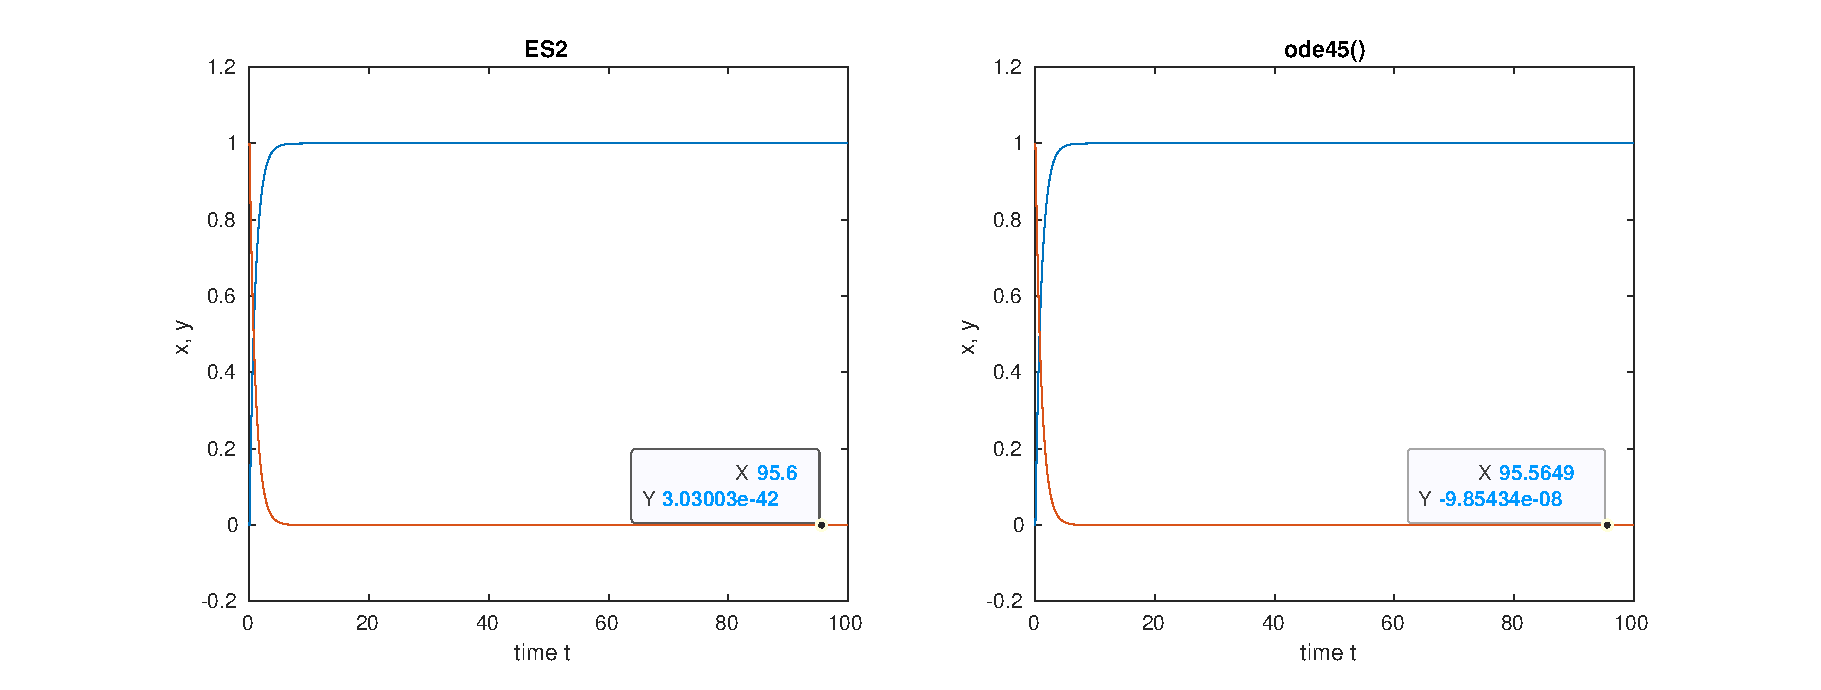
\includegraphics[width = \linewidth]{Matlab/linearproblempositivity.eps}
    \caption{
        Test problem on the system given by Equation \ref{eqn:alineartestproblem}.
        The left figure uses the "ES2" method given by Equation \ref{eqn:secondorderstrangsplittingmethod} taking its $x$ values as opposed to the $z$ values.
        ES2 preserves positivity of the solution throughout.
        The right figure uses MATLAB's \texttt{ode45()} integrator, with a reduced tolerance in order to break positivity.
        The values used were $a=0$ with initial condition $x_0 = 0$, $y_0 = 1$ running for a timespan up to $T = 100$.
        Confusingly the MATLAB graph indexes the horizontal axis $X$ and the vertical $Y$, whereas we plot $x$ and $y$ on the vertical axis against $t$.
        The point labels are necessary to indicate that the MATLAB integrator does not preserve positivity.
    }
    \label{fig:breakposlin}
\end{figure}

Consider the system given by
\begin{equation}
    \frac{\mathrm{d}x}{\mathrm{d}t} = y - ax,~~ \frac{\mathrm{d}y}{\mathrm{d}t} = ax - y
    \label{eqn:alineartestproblem}
\end{equation}
where $a$ is a given constant. This problem is explored briefly for demonstrative purposes in \cite{broekhuizen_biochem_2008}.
The problem admits formulation into the graph-Laplacian form
\begin{equation*}
    \frac{\mathrm{d}}{\mathrm{d}t}\begin{pmatrix}
        x \\
        y
    \end{pmatrix} = \begin{bmatrix}
        -a & 1 \\
        a & -1
    \end{bmatrix} \begin{pmatrix}
        x \\
        y
    \end{pmatrix}
\end{equation*}
where the matrix is constant.

A numerical solution is given in Figure \ref{fig:breakposlin}.
We show that a conventional explicit method, such as the Runge-Kutta method(s) applied in MATLAB's \texttt{ode45()} integrator does not unconditionally preserve positivity.
The formulation of the problem into graph-Laplacian form and the application of a nonnegative initial condition indicates that our solution should preserve positivity, but MATLAB's integrator does not maintain this.
Therefore we have shown that positivity may not be maintained by conventional integrators,
but it is succesful for the ES2 integrator which we know to unconditionally preserve positivity.

\subsection{The Magnus Integrator}

An alternative method suggested in \cite{blanes_pos_2022} is the second order Magnus integrator.
We will first discuss the Magnus expansion \cite{Magnus_1954, blanesmagnus2009}, which allows us to construct this method.
The Magnus expansion considers the linear ODE given by
\begin{equation*}
    \dot{x} = A(t)x
\end{equation*}
with initial condition $x(t=0) = x_0$.
Since $A$ is not time-independent, the exponential solution we have discussed earlier does not hold.
We state that the problem is linear, but the time dependence analogises to the cases we have looked at for a matrix $A(x)$ or $A(t,x)$.
The Magnus expansion considers the solution of this problem to be of the form
\begin{equation*}
    x(t) = \exp(\Omega(t))x_0
\end{equation*}
for some matrix function $\Omega(t)$ which can be expressed in terms of the governing matrix $A$.
We write $\Omega(t)$ as an infinite sum over $\Omega_j(t)$ functions.
From the enclosed sources, we have formulae for these entries.
Specifically, we write
\begin{equation*}
    \begin{aligned}
        \Omega(t) &= \Omega_1(t) + \Omega_2(t) + \mathellipsis = \sum_{j = 0}^{\infty} \Omega_j (t) \\
        \Omega_1(t) &= \int_{0}^{t} A(\tau) \mathrm{d}\tau \\
        \Omega_n(t) &= \sum_{k=1}^{n-1} \frac{B_k}{k!} \int_{0}^{t} S_n^{(j)}(\tau) \mathrm{d}\tau \\
    \end{aligned}
\end{equation*}
where $B_k$ are the Bernoulli numbers \cite{bernoulli} and the $S_n^{(j)}$ functions are defined
\begin{equation*}
    \begin{aligned}
        S_n^{(1)} &= [\Omega_{n-1}, A] \\
        S_n^{(n-1)} &= \operatorname{ad}_{\Omega_1}^{n-1}(A) \\
        S_n^{(j)} &= \sum_{m=1}^{n-j} \left[ \Omega_m, S_{n-m}^{(j-1)} \right] ~~ \text{for}~ 2 \le j \le n-1.
    \end{aligned} 
\end{equation*}
where $\left[\cdot, \cdot\right]$ is the matrix commutator $[A,B] = AB-BA$ and $\operatorname{ad}_A^{j} B = [ A, \operatorname{ad}_A^{(j-1)}B ]$ where $\operatorname{ad}_A^0 B = B$.
We truncate the Magnus expansion to attain an approximation of the solution to a particular order.
Taking just the first term $\Omega_1$, we obtain
\begin{equation*}
    x(t) = \exp\left( \int_{0}^{t} A(\tau) \mathrm{d}\tau \right)x_0
\end{equation*}
which we can approximate with a first order method to get
\begin{equation*}
    x_{n+1} = \exp\left( h A(t) \right)x_n.
\end{equation*}
Note that at a time $\hat{t}$, we can consider $A$ to be a function of $x$ implicitly since $x = x(t)$.
So our previous notions of a problem $\dot{x} = A(x)x$ carry over.
Note also that this first order method is identical to the "exponenial Euler method" we looked at earlier.

The formulation for higher order methods is given in more detail by \cite{blanes_pos_2022} when considering Magnus integrators.
They focus on a second order integrator, for which the autonomous version is given by
\begin{equation}
    x_{n+1} = \exp\left(h A \left( \exp\left(\frac{1}{2}h A(x_n)\right) x_n \right) \right) x_n.
    \label{eqn:secondordermagnus}
\end{equation}
This method uses the midpoint rule in order to form a second order approximation to a formulation of the solution using the first two terms of the Magnus expansion. 

We evaluate the truncation error of the second oder Magnus integrator "EM2", to compare it to our three-exponential "ES2" method.
\begin{equation*}
    \begin{aligned}
        \tau(h) &= x(t_n+h) - \exp \left(
            h A \left( \exp \left(
                \frac{h}{2}A(x_n)
            \right) x_n \right)
        \right) x_n \\
        &= x(t_n + h) - \left(
            I + h A\left(
                \exp \left( \frac{h}{2} A(x_n) \right) x_n
            \right) x_n + \frac{h^2}{2} \left(
                A\left(
                    \exp \left( \frac{h}{2} A(x_n) \right) x_n
                \right)
            \right)^2
        \right) x_n + \mathcal{O}(h^3)
    \end{aligned}
\end{equation*}

% next section is approximating the exponential
\section{Approximating the matrix exponential}
%pade
%the first order approximation
%krylov methods

\subsection{Challenges, series computation}

The positivity preservation methods discussed so far all have one problem in common, being the use of the matrix exponential.
Computing the matrix exponential is significantly expensive, so we hope to introduce some form of approximation by which we can retain a given order of a method.
We might first think to compute the exponential directly from the definition:
\begin{equation*}
    \mathrm{e}^A = I + A + \frac{1}{2}A^2 + \frac{1}{6}A^3 + \mathellipsis = \sum_{j=0}^{\infty} \frac{A^j}{j!}.
\end{equation*}
If we are working in finite precision floating point arithmetic, we can assume that at some point the series will converge such that the sums to $n$ and $n+1$ are represented exactly the same.
In this case, we take the sum to $n$
\begin{equation*}
    \mathrm{e}^A \approx \sum_{j = 0}^{n} \frac{A^j}{j!}.
\end{equation*}
using a modified Horner's form we can express this as
\begin{align*}
	\sum_{j = 0}^{n} \frac{A^j}{j!} &= I + A + \frac{1}{2!}A^2 + \mathellipsis + \frac{1}{n!} A^n \\
	&= I + A\left(
	I + \frac{1}{2} A\left(
			I + \mathellipsis\left(
				\mathellipsis \left( I + \frac{1}{n} A
				\right)
			\right)
		\right)
	\right).
\end{align*}
There are $n$ matrix additions, $n-1$ divisions of a matrix by a scalar and $n-1$ matrix multiplications required to compute this expression.
A multiplication of two $d \times d$ matrices requires $\mathcal{O}(d^3)$\footnote{
    For computer algebra operations, a lower order is better because we often deal with large problems.
    In comparison, we want numerical methods to have higher order because $h$ is often very small.
} floating point operations.
Even with this improvement in efficiency, using this approach to compute a matrix exponential appears expensive.
We will now show that it is also unstable.

The following example is similar to the first demonstration from \cite{moler2003dubious}.
Consider the matrix given by
\begin{equation*}
    A = \begin{bmatrix}
        -121 & 60 \\
        -160 & 79
    \end{bmatrix}.
\end{equation*}
Computing the series form of the exponential directly in double-precision arithmetic sums to $N = 139$ terms, and gives us the solution
\begin{equation*}
    \mathrm{e}_s^A = \begin{bmatrix}
        -2.6531 & -97.1835 \\
        -61.9581 & -184.0359
    \end{bmatrix}.
\end{equation*}
The true form of $A$ can be written as a conjugate transformation
\begin{equation*}
    A = \begin{bmatrix}
        1 & 3 \\
        2 & 4
    \end{bmatrix} \begin{bmatrix}
        -1 & 0 \\
        0 & -41
    \end{bmatrix} \begin{bmatrix}
        1 & 3 \\
        2 & 4
    \end{bmatrix}^{-1}.
\end{equation*}
and so the exponential can be written as 
\begin{equation*}
    e^A = \begin{bmatrix}
        1 & 3 \\
        2 & 4
    \end{bmatrix} \begin{bmatrix}
        \mathrm{e}^{-1} & 0 \\
        0 & \mathrm{e}^{-41}
    \end{bmatrix} \begin{bmatrix}
        1 & 3 \\
        2 & 4
    \end{bmatrix}^{-1} \approx \begin{bmatrix}
        -0.7358 & 0.5518 \\
        -1.4715 & 1.1036
    \end{bmatrix}.
\end{equation*}
Clearly the exponential conputed via series approximation is not an adequate estimate.
% explain the error. moler claims that terms in the sum have magnitudes greater than machine precision of opposite signs, so when adding them we gain terms greater than the final result.

Since this implementation is clearly inadequate, we look for alternative methods for computing the matrix exponential.

\subsection{The Pad\'e Approximation, Scaling and Squaring}

The aim of the Pad\'e approximation for a scalar function $f(x)$ is to construct a rational polynomial approximation to $f$.
The $[n,m]$ Pad\'e approximant for $f$ is the pair $p_{nm}(x), q_{nm}(x)$ which satisfy
\begin{equation*}
    f(x) - \frac{p_{nm}(x)}{q_{nm}(x)} = \mathcal{O}(x^{n+m+1})
\end{equation*} 
where $p_{nm}(x), q_{nm}(x)$ are polynomials.
We generalise this concept to functions on matrices. Given a function $f(A)$, there is a unique $[n,m]$ Pad\'e approximant $R_{mn}(A)$ given by the pair $P_{nm}(A), Q_{nm}(A)$ and formed by $R_{nm}(A) = \left[Q_{nm}(A)\right]^{-1}P_{nm}(A)$
Formulae for Pad\'e approximants for certain matrix functions are known, such as the exponential. 
When computing the product $Q^{-1}P$ we always use a method to solve the system $QX=P$ rather than directly computing the inverse and product.

We said that formulae for the Pad\'e approximation for the exponential are known. From \cite{moler2003dubious} again, we have
\begin{equation}
    \begin{aligned}
        P_{nm}(A) &= \sum_{j=0}^{n} \frac{(n+m-j)!n!}{(n+m)!j!(n-j)!}A^j \\
        Q_{nm}(A) &= \sum_{j=0}^{m} \frac{(n+m-j)!m!}{(n+m)!j!(m=j)!}(-A)^j.
    \end{aligned}
\end{equation}
This is the approximant at zero.
A general Pad\'e approximant is taken about a point, such that it is equal to the approximated function at that point, similar to a Taylor expansion.
In some cases we might take the approximant about a different point, but here zero is no less suitable than anywhere else.

In \cite{blanes_pos_2022} it is stated that the second order diagonal Pad\'e approximation to the exponential is positivity preserving.
This is not true.
This approximation is
\begin{equation*}
    D_{11}(A) = \left[ I - \frac{1}{2}A \right]^{-1} \left[ I + \frac{1}{2} A\right].
\end{equation*}
Consider the matrix given by
\begin{equation*}
    A = \begin{bmatrix}
        -4 & 1 & 0 \\
        2 & -1 & 2 \\
        2 & 0 & -2
    \end{bmatrix}
\end{equation*}
and vector
\begin{equation*}
    x = \begin{bmatrix}
        3 \\
        1 \\
        2
    \end{bmatrix}.
\end{equation*}
To four significant figures the product of the exponential with the vector is
\begin{equation}
    \mathrm{e}^{A} x = \begin{pmatrix}
        0.9422 \\
        3.8506 \\
        1.2071
    \end{pmatrix}
\end{equation}
so positivity is preserved. However if we compute the $[1,1]$ Pad\'e approximant and compute the product we obtain
\begin{equation*}
    \left[D_{11}(A)\right]x = \left[ I - \frac{1}{2}A \right]^{-1} \left[ I + \frac{1}{2}A \right] x = \begin{pmatrix}
        -0.0167 \\
        1.1500 \\
        0.3667
    \end{pmatrix}
\end{equation*}
where we fail to preserve positivity.
A method is proposed in which we exploit the properties of the exponential by writing $A = \bar{A} + \hat{a}I$, such that $\bar{A}$ is entirely nonnegative.
Then
\begin{equation*}
    \mathrm{e}^A = \mathrm{e}^{\bar{A} + \hat{a}I} = \mathrm{e}^{\hat{a}} \mathrm{e}^{\bar{A}}
\end{equation*}
and we compute the $[1,1]$ Pad\'e approximant for $\bar{A}$.
In our example $\hat{a} = -4$ and
\begin{equation*}
    \mathrm{e}^{\hat{a}} [D_{11}(\hat{A})] x = \begin{bmatrix}
        0.5833 \\
        1.7500 \\
       -0.8333
    \end{bmatrix}.
\end{equation*}
So clearly the second order Pad\'e method does not preserve positivity.



\section{Optimisation Methods}

% mass preservation can be recovered from clipping using an optimisation algorithm

% balancing the weights of a RK method - the added constraint enforces positivity


\section{Special Cases}

% the third order method from that chinese paper

% backward Euler





\end{document}